% -*- root: ../../main.tex -*- %

\section{Preliminary decisions} % (fold)
\label{sec:design_decisions}
  All of the variants highlighted in \ref{sub:promising_combinations_of_characteristics} represent interesting approaches for the utilization of Docker for the enactment of workflows for different use cases.
  For this prototype, $G_{DV}^{SEPC}$ with a partially integrated workflow engine is the implemented variant for several reasons. First and foremost, this combination enables the use of basic Docker commands for the suspension and continuation of a workflow and single activities, as described in \ref{ssub:element_wrapping_containers}. Second, $*_{*}^{SEPC}$ leverages the already existing communication between the local daemon of a node and the swarm master daemon to publish the status of both workflow instances and activity instances, in the form of events concerning container statuses. Third, $G_{DV}^{*}$ is a promising variant for the demonstration of  various scheduling mechanisms introduced in \ref{sub:execution_scheduling}, since this variant includes implicit affinities by default. While partially integrating the workflow engine is mainly interesting for its role in the previously mentioned native pausing, it also facilitates the working directory management, as argued in \ref{ssub:element_wrapping_containers}.

  The services are implemented using \emph{Ruby}, a dynamically typed object-oriented programming language. Ruby provides the means to write concise, well readable code \cite[p.~782]{Nanz2015Comparative}. It is by no means the language with the best performance \cite[p.~786]{Nanz2015Comparative}. However, the focus of this thesis is to explore conceptual possibilities rather than developing efficient implementations of them. An emphasis is thus put on the expressiveness of the used language to help the reader to grasp the underlying concept quickly.

  All services that require access to any Docker \ac{API} do so by using a gem called \texttt{docker-api}, which provides a client for these \acp{API}. \emph{Gem} is the name for distributable packages in the Ruby ecosystem. These packages can be managed using \emph{Gemfiles}, in which the package dependencies of an application may be declared.

  The Ruby-based web application framework \ac{RoR} is used for the implementation of the developer gateway and user gateway. It qualifies for this task because it comes with several functionalities that aim at the fast creation of prototypes. For example, so called \emph{scaffolds} permit the creation of model and controller classes and appropriate views based on a specified database schema; the included library \emph{ActiveRecord} supports adding object-relational mapping functionality to model classes \cite[p.~5]{Jazayeri2007Some}.

  ActiveRecord is also used in those services that do not use Rails but need to store objects in databases, namely in the \texttt{definition}, \texttt{organization}, and \texttt{worklist} services.

  For this prototype, RabbitMQ was chosen as message oriented middleware, because it is well documented and provides a web interface for monitoring and administration.
  The gems \texttt{Hutch} and \texttt{Bunny} provide different levels of abstraction for the interaction with the RabbitMQ message queue. \texttt{Hutch} itself is based on \texttt{Bunny} and imposes some opinionated conventions for the use of the message queue, as well as automatic (de-)serialization of the messages' payload.

% section design_decisions (end)

\section{Execution Images} % (fold)
\label{sec:execution_images}
  \begin{figure}[htbp]
    \centering
    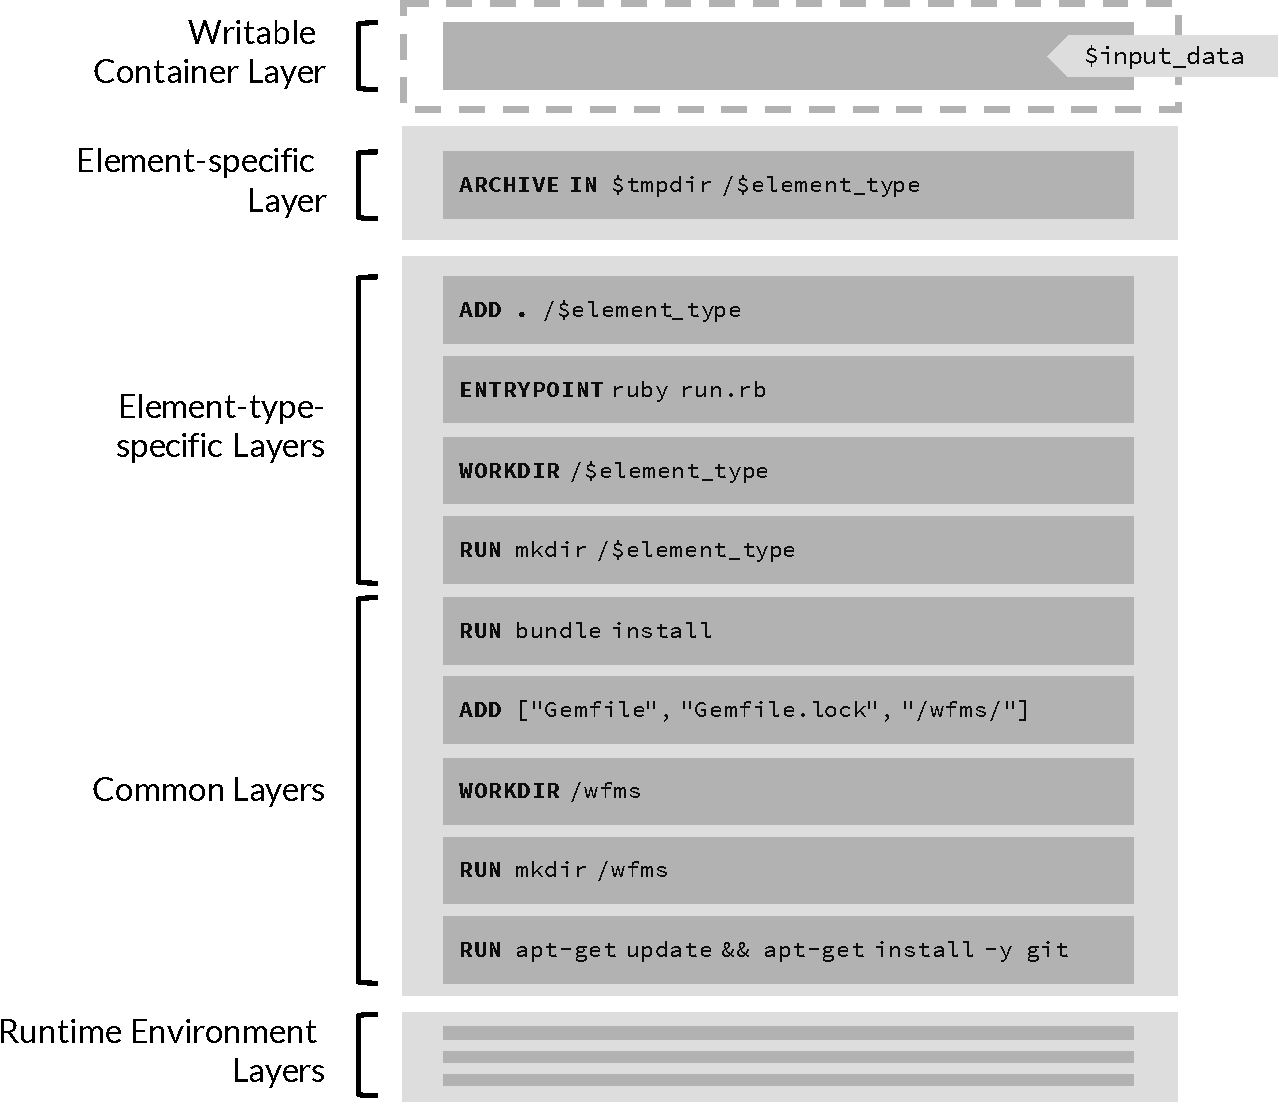
\includegraphics[width=0.95\textwidth]{content/images/execution_container-crop.pdf}
    \caption{Layer Contents for Element-wrapping Containers}
    \label{fig:detailed_layers_for_element_wrapping_containers}
  \end{figure}

  \subsection{Workflow Image} % (fold)
  \label{sub:workflow_container}
    The workflow image is structured as planned in \ref{sub:workflow_activity_images}. The runtime-environment layers are provided by inheriting all layers of the \texttt{ruby:2.2} image. On top of these, common layers are created, in which the required gems are installed. Then, the \texttt{/workflow} directory is created, into which the required Ruby files are copied. The file \texttt{run.rb} is set as the default command.

    The workflow instance is structured as depicted in \ref{fig:uml_class_diagram_wf_base}. The \texttt{run} script loads the required dependencies and ensures, that the container is connected to the \texttt{enactment} network. Then, it initiates the enactment by creating an instance of the \texttt{ProcessInstance} class and calling its start method.

    - application
      - process instance
      - process definition
      - activity instance
      - file helper
      - configuration
    - dirs
      - /workflow
        - process definition.json
        - input.mapping.json
        - input.schema.json
        - workflow.info.json

  % subsection workflow_container (end)

  \subsection{Activity Image} % (fold)
  \label{sub:activity_containers}
    - application
      - configuration
      - file helper
    - dirs
      - /activity
        - input.mapping.json
        - input.schema.json
        - activity.info.json

    - application wrapper
    - manual input wrapper
    - custom code wrapper
  % subsection activity_containers (end)
% section execution_images (end)

\section{System Components} % (fold)
\label{sec:components_implementation}
  \subsection{Workflow Definition Service} % (fold)
    \label{sub:workflow_definition_service}

    The workflow definition service is composed of three components: one container running a Ruby on Rails application which is configured to expose a JSON API, one container running a PostgreSQL database and a data volume container which provides persistent storage to that database.

    PostgreSQL was chosen as database solution for the definition service, because it supports both relational data, which is useful for storing the workflow, its elements and their relations, and the document-store-like JSONB format, which allows the schema-less storage of configuration information.
    - useful for queryable conf with dynamic structure
    In order to keep the stored data during container restarts or migrations across nodes, the database makes use of a data volume container which provides its working directory.

    The application container is granted access to the Docker daemon of its host node in form of a mounted volume in order to build and push images.

    As planned in \ref{subs:workflow_definition_service}, the service has the model classes \texttt{Activity}, \texttt{ControlFlow}, \texttt{ProcessDefinition} and \texttt{Workflow}, which on the one hand act as object-relational mappers for persistence to the database, on the other hand ensure some validity constraints. Further, there exists a controller class for each of the aforementioned models, which provides \ac{CRUD} actions for the respective model. In order to have more fine-grained control over the serialization of a workflow, the \texttt{WorkflowFullSerializer} is used if a specific workflow is requested. It nests all relevant workflow elements into the workflow model before it is serialized.

    While the modeling logic is partially explicitly contained in the model and controller classes and implicitly in the underlying data schema, the export logic resides in the classes \texttt{ImageManager} and \texttt{ImageBuilder}, which are supported by the class \texttt{ProcessDefinitionImageSerializer}.

    The \texttt{ProcessDefinitionImageSerializer} provides the means to create the consolidated JSON representation of a process definition with all information that is necessary to execute the corresponding workflow. An example for the serialized output can be seen in Figure~\ref{fig:exported_process_definition_in_json_format}.

    \subsubsection{Export of a Workflow} % (fold)
      \label{ssub:exporting_a_workflow}
      If the user requests the export of a workflow, the request is forwarded to the \texttt{ImageManager}.
      In order to export a workflow, the first step is to identify all of its elements that require to be wrapped in an image. Obviously, one of them is the workflow itself. The other required images are determined by traversing the workflow's process definition recursively. Each activity has to be exported, too, and each sub-workflow has a method that exposes the Docker images it requires beyond that. It does so by passing the call for required images on to the referenced workflow, which collects its required images analogously, and returning the result.

      The \texttt{ImageBuilder} then iterates over all these elements and creates a correspondent image for each. Starting with the respective base image -- \texttt{ac\_base} or \texttt{wf\_base} -- it adds additional layers to do so. The \texttt{ImageBuilder} creates the files which are specific to the current element from the activity's or workflow's configuration, \ie the input/output validation schemata, the element's description file, and in case of a workflow the serialized process definition, in a temporary directory. The \texttt{ImageBuilder} then copies these files to the image and names it after the workflow element that it represents.

      The \texttt{ImageManager} then uploads all images that were successfully built to the private repository and publishes a notification of the successful build via the message broker.
      % subsubsection exporting_a_workflow (end)
    % subsection workflow_definition_service (end)

  \subsection{Organization Management Service} % (fold)
    \label{sub:organization_management_service}
      The organization management service is built similar to the workflow definition service. Just like it, the service consists of three Docker containers: a \ac{RoR}-based application that is backed by a PostgreSQL database with a data volume.

      As visible in Figure~\ref{fig:uml_class_diagram_organization}, the application itself is simpler than that of the workflow definition service, though. It merely consists of the classes User and Role and their respective controller classes. The RoleController offers an additional method to draw one user form all users with a certain role at random, which can be used as a rudimentary way to distribute tasks among users.

      The organization management service publishes successful CRUD events on the models to the message broker, such that the other services can react to it.

    \begin{figure}[htbp]
      \centering
      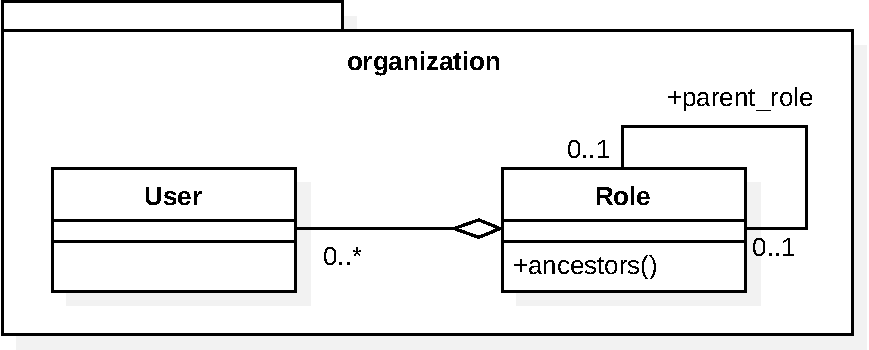
\includegraphics[width=0.65\textwidth]{content/images/class_diagram_organization-crop.pdf}
      \caption*{\scriptsize Note: Controllers omitted for the sake of simplicity. User and Role both have a controller with the respective pluralized name plus a `Controller' suffix.}
      \caption{UML Class Diagram for the Organization Service}
      \label{fig:uml_class_diagram_organization}
    \end{figure}
    % subsection organization_management_service (end)

  \subsection{Worklist Service} % (fold)
    \label{sub:worklist_service}
      The worklist service is even simpler than the organization management service. It consists of three Docker containers of the same kind, too. It only features one model class and its corresponding controller: the \texttt{WorklistItem} and the \texttt{WorklistItemController}.

      Worklist items may be queried by the identifier of the assigned user. They contain a JSON schema that describes the expected data and, after they have been worked on, the data itself.

      TODO
      % - reacts to
      %   - user created/deleted/updated
      %   - workflow finished
      %     - remove
    % subsection worklist_service (end)

  \subsection{Workflow Engine Service} % (fold)
    \label{sub:workflow_engine_service}
      - application
    % subsection workflow_engine_service (end)

  \subsection{Developer Gateway} % (fold)
    \label{sub:developer_gateway}
      The developer gateway does not require any database, as it merely forwards requests to the \ac{MOM}. Hence, it consists of a single Docker container that wraps a \ac{RoR} application.

      In order to be reachable by its users, this container needs to expose the port of the application to the host's network.

      \subsubsection{Backend} % (fold)
      \label{ssub:backend}


      % subsubsection backend (end)

      \subsubsection{Frontend} % (fold)
        \label{ssub:frontend}
          - forms for data manipulation
          - visual workflow modeling
          - infrastructure:
            - display available nodes + ip
            - display installed images and running containers

        % subsubsection frontend (end)
    % subsection developer_gateway (end)

  \subsection{User Gateway} % (fold)
    \label{sub:user_gateway}
    Just like the developer gateway, the user gateway does not require any storage mechanism. It thus also consists of only one Docker container, which contains the \ac{RoR} application.

    - must expose ports

      - application
        - backend: rails
        - frontend: angular app
    % subsection user_gateway (end)

  \subsection{Message Oriented Middleware} % (fold)
    \label{sub:message_oriented_middleware}
      RabbitMQ exists as a pre-configured Docker image (\texttt{rabbitmq}) on the Docker Hub and can thus be utilized easily. The configuration of RabbitMQ in this image takes place when the respective container is run, which allows its configuration in the \texttt{docker-compose} configuration file as depicted in Figure~\ref{fig:configuration_of_the_mom_service_in_the_docker_compose_file}.
      For the sake of simplicity, no authentication mechanism was introduced besides the simple default username/password combination. As the central point of communication, the \ac{MOM} is the only container which is connected to all three overlay networks. While one would probably avoid exposing this service in a real world use case, it is exposed to the host's network for its use in a prototype, as this allows to monitor the messaging activity of the services.

      ** TODO constraints **
      \begin{figure}[!htbp]
        \inputminted[firstline=23,lastline=33,fontsize=\footnotesize,linenos=true,numberblanklines=true,showspaces=false,breaklines=true,baselinestretch=1]{yaml}{../code/wfms.yml}
        \caption{Configuration of the \ac{MOM} service in the Docker Compose file}
        \label{fig:configuration_of_the_mom_service_in_the_docker_compose_file}
      \end{figure}
    % subsection message_oriented_middleware (end)

  \subsection{Infrastructure Management Service} % (fold)
    \label{sub:infrastructure_management_service}
      The data that this service offers -- the state of the Docker swarm and its nodes -- should be up-to-date. It is thus gathered ad-hoc when a request arrives. This proceeding makes a database obsolete, that is why the infrastructure management service solely consists of one Docker container which contains the application.

      The \texttt{EnvironmentManager} queries the Docker daemon and processes the response. It is supported by the \texttt{DockerHelper}, which provides the means to point the local Docker client at arbitrary members of the swarm or the swarm manager.

      % It could be argued, that requests to the swarm could be made directly in the developer gateway backend. This, however, would counter the \ac{MSA} principle. In case that the Docker service alters the way it returns information, the adaption to it would require

      % -- It could be argued that the functionality could also be implemented in the developer gateway, but
      %   - separation of tasks, can be adapted independently if docker API changes

      The infrastructure management service
      - application
        - app logic
          - docker helper
          - environment manager
        - controllers
          - servers controller
        - models
          - server

    % subsection infrastructure_management_service (end)

  \subsection{Registry} % (fold)
    \label{sub:registry}
    A local registry is deployed in its own container in order to distribute the created images.
    Docker provides the \texttt{registry} image for this purpose, of which the version \texttt{registry:2.3} is used, since it is the newest stable version at the time of this writing.

    The registry is configured to be restarted automatically in case that itself or the node it runs on fails. Further, it is exposed on the host's network do make it reachable for all nodes in the swarm. This is necessary, as their daemons are no containers and thus cannot be connected to the overlay network. Consequentially, it is configured in the \ac{WfMS}' Docker Compose file as follows:

    \begin{figure}[!htbp]
      \inputminted[firstline=12,lastline=21,fontsize=\footnotesize,linenos=true,numberblanklines=true,showspaces=false,breaklines=true,baselinestretch=1]{yaml}{../code/wfms.yml}
      \caption{Configuration of the registry service in the Docker Compose file}
      \label{fig:configuration_of_the_registry_service_in_the_docker_compose_file}
    \end{figure}
    % subsection registry (end)

  \subsection{Provisioning Service} % (fold)
    \label{sub:provisioning_service}
      - application
    % subsection provisioning_service (end)
% section components (end)


\section{Exemplary Deployment} % (fold)
\label{sec:exemplary_deployment}

  - 4 VMs

  The deployment of all services is performed using Docker Compose, as this tool provides some conveniences for deployment-related tasks.
  First, Docker Compose enables the automatic building, starting, stopping and removal of the services' images, as described in \ref{sub:docker_compose}.
    **  - build w/ image name
        - build on specifc node
        - up command
          - build missing images
          - start stopped/missing containers
          - recreate containers with changed images
          - ignore existing containers

  Second, the configuration of all services and the required networks that connect them may be specified in a single \emph{YAML} file. \ac{YAML} is designed with a focus on human readability \cite{Kiki2009Yaml}. The configuration file may thus serve as a textual documentation of the system's architecture.

  - deployment as in Figure~\ref{fig:deployment_diagram_of_the_architecture}
  - not really WAN, not really LAN -> exemplary


  \begin{figure}[htbp]
    \centering
    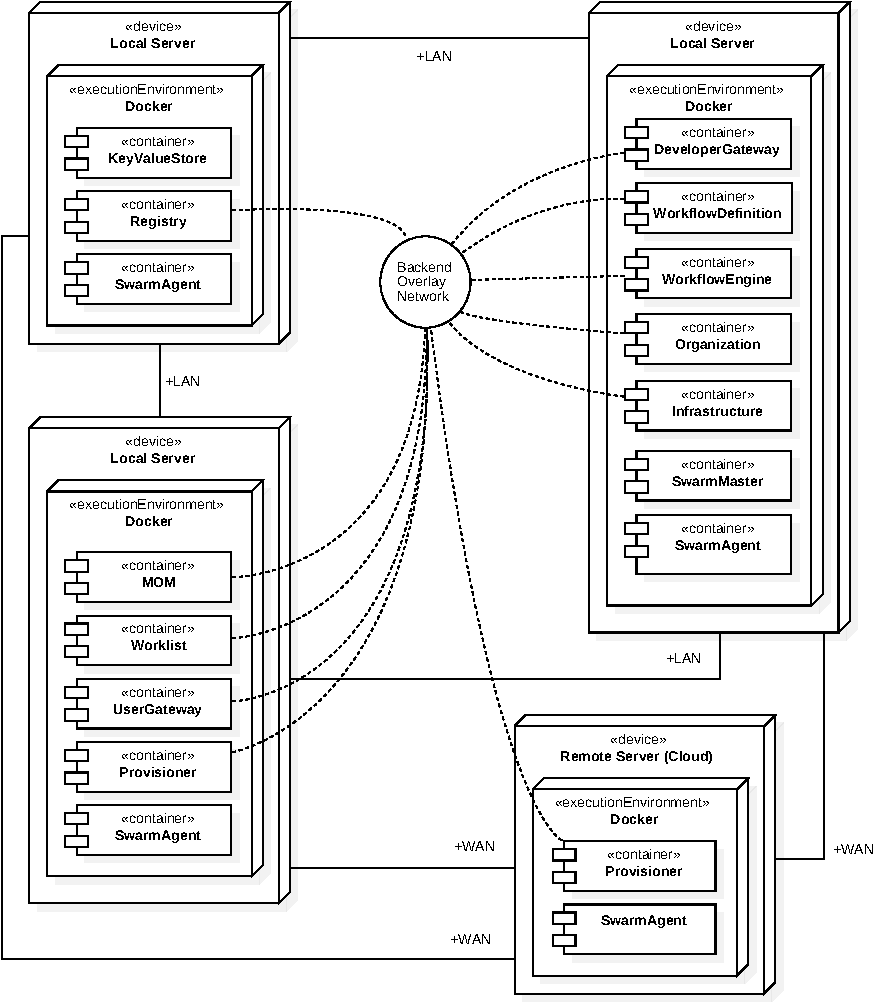
\includegraphics[width=0.95\textwidth]{content/images/Architecture-crop.pdf}
    \caption*{\scriptsize Note: the depicted distribution of containers to nodes is just exemplarily. Most of them could run on any node in the swarm. The only mandatory assignments are the swarm agents, of which each node needs one, and the provisioners, of which each node that is intended to execute workflows on needs one. \\ Also, the databases and their respective data volumes were omitted for the sake of clarity.}
    \caption{Deployment Diagram of the Architecture}
    \label{fig:deployment_diagram_of_the_architecture}
  \end{figure}
  -
% section exemplary_deployment (end)

\section{Implementation Issues and compromises} % (fold)
  - gateways are synchronous to keep them simple
    - no concurrent requests made

  -ruby: requires run env: large images
\label{sec:implementation_issues}

% section implementation_issues (end)
